% This is samplepaper.tex, a sample chapter demonstrating the
% LLNCS macro package for Springer Computer Science proceedings;
% Version 2.21 of 2022/01/12
%
\documentclass[runningheads]{llncs}
%
\usepackage[T1]{fontenc}
% T1 fonts will be used to generate the final print and online PDFs,
% so please use T1 fonts in your manuscript whenever possible.
% Other font encondings may result in incorrect characters.
%
\usepackage{graphicx}
\usepackage{url}
\usepackage{hyperref}
% Used for displaying a sample figure. If possible, figure files should
% be included in EPS format.
%
% If you use the hyperref package, please uncomment the following two lines
% to display URLs in blue roman font according to Springer's eBook style:
%\usepackage{color}
%\renewcommand\UrlFont{\color{blue}\rmfamily}
%\urlstyle{rm}
%

\usepackage{amsmath}

\usepackage{xcolor}

% ragged-right fixed-width table columns (avoids stretched inter-word gaps)
\usepackage{array}

% let grouped tables/figures fill more of a page so they place cleanly
% instead of drifting far from their reference
\renewcommand{\topfraction}{0.9}
\renewcommand{\bottomfraction}{0.8}
\renewcommand{\textfraction}{0.07}
\renewcommand{\floatpagefraction}{0.75}
\setcounter{topnumber}{3}
\setcounter{totalnumber}{4}

% number subsubsections so the supervised/unsupervised parts within the
% Machine Learning Analysis section are individually referenceable
\setcounter{secnumdepth}{3}

% allow line breaks after underscores so long snake_case identifiers in
% \texttt{} (e.g. carry_spread_levered) wrap instead of overflowing the margin
\makeatletter
\let\origunderscore\_
\renewcommand{\_}{\origunderscore\allowbreak}
\makeatother

\begin{document}

\title{Recursive Leverage in Yield-Bearing Stablecoins: Proof-of-Concept and Empirical Analysis}

\titlerunning{Recursive Leverage in Yield-Bearing Stablecoins}

\author{Igli Kristo\inst{1} \and
Dawid Rymarczyk\inst{1} \and
Claudio J. Tessone\inst{1}\thanks{Advisor} \and
Krzysztof M. Gogol\inst{1}\thanks{Assistant-Advisor}}

\institute{University of Zurich, Switzerland}

\maketitle              % typeset the header of the contribution
%
\begin{abstract}
    \input{sections/00Abstract.tex}
\keywords{DeFi \and Yield-Bearing Tokens \and Recursive Leverage \and Ethereum \and Machine Learning}
\end{abstract}

\section{Introduction}
\label{sec:intro}

This project empirically studies how large holders use yield-bearing tokens (YBTs) to construct recursive looping strategies across Ethereum mainnet lending protocols. A YBT accrues yield passively through staking, lending, or vault returns while also serving as collateral. Some large holders exploit this dual property by depositing a YBT, borrowing against it, acquiring additional exposure, and repeating the process to increase effective carry at the cost of higher liquidation risk.

\subsection{Motivation}

Despite the rapid growth of yield-bearing stablecoins, limited empirical research characterises how large holders deploy these tokens. Understanding leverage depths and rebalancing behaviours is critical for systemic risk assessment, protocol parameter calibration, and on-chain risk monitoring, as concentrated leveraged positions can trigger cascading liquidations during market stress.

\subsection{Problem Statement}

The primary contribution is an empirical characterisation of strategy archetypes among large YBT holders. A secondary contribution is testing whether on-chain risk indicators can predict short-horizon rebalancing and stressed risk states.

\subsection{Research Questions}

\begin{itemize}
    \item \textbf{RQ1:} What recurring leverage and looping strategy archetypes can be identified among large holders of major yield-bearing stablecoin tokens on Ethereum mainnet?
    \item \textbf{RQ2:} Which observable risk-management characteristics (leverage depth, collateral buffers, and rebalancing behaviour) differentiate these archetypes?
    \item \textbf{RQ3:} To what extent can on-chain state variables predict short-horizon rebalancing events and stressed risk states?
\end{itemize}

\subsection{Contributions}

This work makes the following contributions:
\begin{itemize}
    \item A proof-of-concept bot demonstrating recursive leverage strategies on Morpho Blue, implemented with and without flashloans.
    \item A data collection pipeline identifying large YBT holders and their on-chain activity across Aave v3, Morpho Blue.
    \item An empirical analysis of strategy archetypes and risk management behaviours among whale addresses.
\end{itemize}

\subsection{Paper Organisation}

Section~\ref{sec:background} provides background on yield-bearing tokens and lending protocols. Section~\ref{sec:poc} describes the proof-of-concept leverage bot. Section~\ref{sec:data} details the data collection pipeline. Section~\ref{sec:feature-engineering} covers feature engineering. Section~\ref{sec:ml-analysis} presents the machine learning analysis. Section~\ref{sec:discussion} discusses findings and limitations, and Section~\ref{sec:conclusions} concludes.

\section{Background}
\label{sec:background}

This section introduces yield-bearing tokens, the lending protocols where they are used as collateral, and the recursive leverage strategy known as looping.

\subsection{Yield-Bearing Tokens}

Yield-bearing tokens (YBTs) are ERC-20 tokens whose value accrues over time relative to an underlying asset through staking, lending, or vault returns. Unlike static stablecoins such as USDC or USDT, YBTs automatically compound yield into the token's exchange rate. The ERC-4626 standard provides a uniform interface for these tokenised vaults, defining methods for deposit, withdrawal, and share conversion.

As of Q1 2026, major USD-denominated YBTs include sUSDe (Ethena, approximately \$3.5B market cap), sUSDS (Sky, approximately \$6B), and syrupUSDC (Maple Finance, approximately \$1.8B). These tokens generate yield through staking rewards, savings rate mechanisms, or institutional lending, typically offering 4--8\% APY.

\subsection{Lending Protocols}

Three major Ethereum mainnet lending protocols support YBTs as collateral:

\textbf{Aave v3} is a pooled lending protocol where depositors supply assets to shared liquidity pools and borrowers draw from these pools. Each asset has protocol-defined parameters including loan-to-value (LTV) ratios and liquidation thresholds. Aave governance controls which assets can be listed and what parameters they use.

\textbf{Morpho Blue} is a permissionless lending protocol that uses isolated markets where each collateral-borrow pair operates independently. Unlike Aave, anyone can create a new market with any collateral and borrow asset without requiring governance approval. This design allows for higher LTV ratios on specific pairs, as risk is contained within each market rather than shared across the protocol.

\subsection{Recursive Leverage (Looping)}

Looping refers to a recursive leverage strategy where the holder deposits a yield-bearing token as collateral, borrows a stablecoin against it, uses the borrowed stablecoin to purchase more of the same yield-bearing token, and re-deposits it as additional collateral. This cycle can be repeated to amplify effective carry at the cost of proportionally higher liquidation risk.

The profitability of looping depends on the carry spread: the difference between the YBT yield and the borrowing cost. A positive spread means the position earns more than it pays in interest. A negative spread means the operator is losing money and should unwind.

\subsection{Related Work}

Prior work on DeFi leverage has examined liquidation cascades and systemic risk in lending protocols. Qin et al.\ studied empirical liquidation patterns on Compound and Aave, finding that cascading liquidations can amplify market stress. Studies of on-chain behavioural analysis have used clustering techniques to identify strategy archetypes among DeFi participants. This work extends that literature by focusing specifically on recursive leverage strategies in yield-bearing stablecoins, a segment that has grown rapidly but remains underexplored empirically.

\section{Proof-of-Concept}
\label{sec:poc}

This section describes the proof-of-concept bot developed to demonstrate and validate recursive leverage mechanics on a real blockchain. The bot operates on Base mainnet using the yoUSD/USDC market on Morpho Blue.

\subsection{Design Goals}

The purpose of the proof-of-concept is to demonstrate recursive leverage mechanics on a live chain before analysing whale behaviour on Ethereum mainnet. The bot validates the looping process end-to-end: depositing capital, supplying collateral, borrowing against it, and repeating the cycle to amplify exposure.

We deploy on Base rather than Ethereum mainnet to minimise gas costs during development and testing. Base is an Ethereum Layer-2 with significantly lower transaction fees while maintaining compatibility with mainnet contracts. The empirical analysis in later sections uses Ethereum mainnet data due to higher capital concentration, deeper liquidity, and longer transaction histories.

We selected yoUSD as the yield-bearing token because it is fully permissionless (no whitelist), implements the ERC-4626 vault standard for simple deposit and redemption, offers approximately 8\% native APY paid in USDC, and has a confirmed Morpho Blue market on Base with 91.5\% liquidation LTV.

Ownership of the deployed contract is transferred to a 1-of-2 Gnosis Safe multisig wallet. This separation of deployment signer and operational signer provides higher security and allows the use of Gnosis Safe's transaction builder for complex operations.

\begin{figure}[h]
\centering
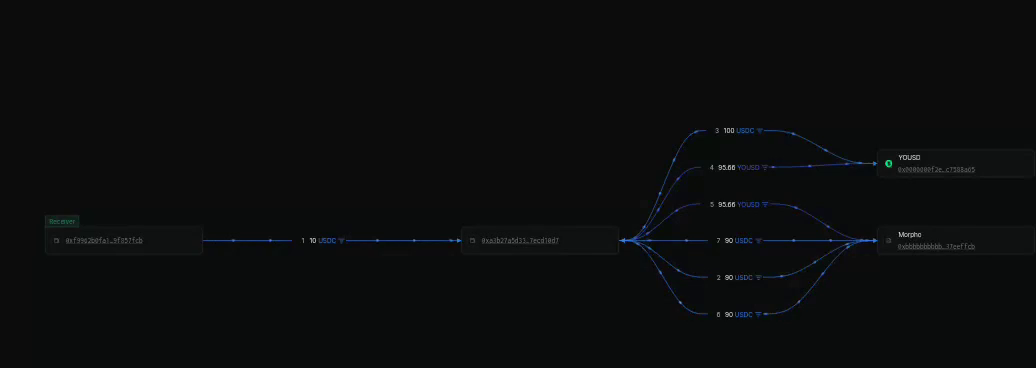
\includegraphics[width=\textwidth]{figures/leverage-flow.png}
\caption{Execution flow of the flashloan-based leverage strategy, visualised via Tenderly.\protect\footnote{\url{https://dashboard.tenderly.co/public/safe/safe-apps/simulator/7fb53629-e928-45d1-830b-9dc967b76ccc/fund-flow}}}
\label{fig:leverage-flow}
\end{figure}

\subsection{Strategy 1: Flashloan-Based Leverage}

The first strategy uses a Morpho flashloan to build the entire leveraged position atomically in a single transaction. This approach is implemented in the \texttt{LeverageBot.sol} smart contract.

The execution flow proceeds as follows:
\begin{enumerate}
    \item The owner approves 10 USDC and calls \texttt{execute()}.
    \item The contract pulls 10 USDC from the owner, then requests a 90 USDC flashloan from Morpho.
    \item Morpho calls back \texttt{onMorphoFlashLoan()}; the contract now holds 100 USDC.
    \item The contract deposits all 100 USDC into the yoUSD vault, receiving approximately 93 yoUSD shares.
    \item The contract supplies yoUSD as collateral on Morpho in the yoUSD/USDC market.
    \item The contract borrows 90 USDC against the yoUSD collateral.
    \item The contract repays the 90 USDC flashloan; the transaction completes.
\end{enumerate}

The result is approximately 100 USDC worth of yoUSD collateral with 90 USDC of debt, funded with only 10 USDC of the owner's capital. This represents roughly 10x leverage.

The \texttt{unwind()} function reverses this process atomically: it flashloans enough USDC to repay the debt, withdraws all yoUSD collateral, redeems yoUSD back to USDC, repays the flashloan, and sweeps any remaining USDC (original capital plus accrued yield) to the owner.

\subsection{Strategy 2: Iterative Looping}

The second strategy requires no smart contract. It uses a JavaScript script that loops step-by-step across multiple transactions:
\begin{enumerate}
    \item Deposit USDC into yoUSD vault, receive yoUSD shares.
    \item Supply yoUSD as collateral on Morpho.
    \item Borrow 88\% of the collateral value back as USDC.
    \item Repeat with the borrowed USDC.
\end{enumerate}

The script executes three loops by default, building up leverage incrementally. If any loop fails, the script automatically triggers \texttt{unwind.js} to clean up the partial position.

This approach is slower (multiple transactions incur multiple gas fees) but simpler to understand and debug. It also demonstrates the manual process that many whale addresses use, as observed in the empirical data.

\subsection{Security Considerations}

Several security measures are implemented:

\textbf{Ownership model.} The contract uses an \texttt{onlyOwner} modifier for privileged functions (\texttt{execute}, \texttt{unwind}, \texttt{rescueToken}). Ownership is transferred to a Gnosis Safe after deployment.

\textbf{Flashloan callback guard.} The \texttt{onMorphoFlashLoan} callback is protected by an \texttt{onlyMorpho} modifier, ensuring only Morpho can invoke it.

\textbf{Rescue function.} A \texttt{rescueToken} function allows the owner to recover any tokens accidentally sent to the contract.

\textbf{Atomic execution.} The flashloan strategy executes entirely within a single transaction. If any step fails, the entire transaction reverts, leaving no partial state.

\subsection{Deployment and Testing}

The contract is deployed on Base mainnet at address \texttt{0xa3B27a...Ecd10d7}, with ownership transferred to a 1-of-2 Gnosis Safe at \texttt{0xf9962B...857fCb}. Full addresses are recorded in the deployment artefacts.

\textbf{Operational workflow.} To execute the leverage strategy via the Safe, the operator uses the Gnosis Safe Transaction Builder:
\begin{enumerate}
    \item Create a new transaction, paste the USDC contract address on Base, and let the interface auto-generate the ABI.
    \item Call \texttt{approve()} with the bot address as spender and 10 USDC as the amount. This is a one-time approval.
    \item Create a second transaction targeting the bot contract and call \texttt{execute()}.
    \item Optionally simulate the transaction via Tenderly to preview the fund flow before signing.
    \item Sign and execute the transaction through the Safe.
\end{enumerate}

The Tenderly simulator provides a visual flowchart animation showing the complete execution path: USDC transfer, flashloan request, yoUSD deposit, collateral supply, borrow, and flashloan repayment (Figure~\ref{fig:leverage-flow}).

\textbf{Testing.} Tests run against a real Base fork using Hardhat, with no mocks or stubs. The test suite covers:
\begin{itemize}
    \item Execution flow and position state verification
    \item Ownership transfer and access control
    \item Unwind functionality and USDC recovery
    \item Flashloan callback guards
    \item Full lifecycle via Safe-impersonated transactions
\end{itemize}

All contract addresses are recorded in \texttt{deployments/LeverageBot\_base\_latest.json}. The full contract code is provided in Appendix~\ref{sec:code}.

\section{Data Collection}
\label{sec:data}

This section describes the data collection pipeline for yield-bearing token activity and whale identification across Ethereum mainnet lending protocols.

\subsection{Token Selection}

Three USD-denominated yield-bearing tokens were selected based on the following criteria: top candidates by Ethereum mainnet circulating value and TVL, minimum on-chain liquidity threshold, minimum active holder count, active integration as collateral on at least one major lending protocol, and activity throughout the sample period.

\begin{table}[h]
\centering
\caption{Selected yield-bearing tokens.}
\label{tab:tokens}
\begin{tabular}{llll}
\hline
\textbf{Token} & \textbf{Issuer} & \textbf{Market Cap} & \textbf{Typical APY} \\
\hline
sUSDe & Ethena & \$3.5B & 4--8\% \\
sUSDS & Sky & \$6B & 4--6\% \\
syrupUSDC & Maple Finance & \$1.8B & 5--8\% \\
\hline
\end{tabular}
\end{table}

These tokens represent the largest USD-denominated yield-bearing stablecoins on Ethereum mainnet with active lending protocol integrations.

\subsection{Protocol Coverage}

Three lending protocols are covered based on where these tokens are actively used as collateral.

\begin{table}[h]
\centering
\caption{Protocol coverage by token.}
\label{tab:protocols}
\begin{tabular}{lcc}
\hline
\textbf{Token} & \textbf{Aave v3} & \textbf{Morpho Blue} \\
\hline
sUSDe & Yes & Yes \\
sUSDS & No & Yes \\
syrupUSDC & No & Yes \\
\hline
\end{tabular}
\end{table}

\subsection{YBT Scraper}

The YBT scraper collects metadata, prices, and protocol events for the three tokens under study. Data is sourced from DeFiLlama (TVL, APY) and Dune Analytics (prices, events).

\begin{table}[h!]
\centering
\caption{YBT scraper output files.}
\label{tab:ybt-output}
\begin{tabular}{lp{7cm}}
\hline
\textbf{Output File} & \textbf{Contents} \\
\hline
\texttt{ybt\_metadata.json} & Token name, issuer, address, decimals, TVL, APY \\
\texttt{ybt\_prices.csv} & Daily average, low, and high prices for depeg monitoring \\
\texttt{aave\_events.csv} & Supply, withdraw, borrow, repay, liquidation events (sUSDe) \\
\texttt{morpho\_events.csv} & Events for all three tokens on Morpho Blue \\
\hline
\end{tabular}
\end{table}

Each event record includes timestamp, block number, transaction hash, user address, and amount.

\subsection{Whale Identification}

The whale identification pipeline finds the top addresses per token per protocol that have actively engaged in looping or flashloan strategies, ranked by lifetime token volume.

\textbf{Pipeline:}
\begin{enumerate}
    \item Run Dune SQL queries per token per protocol, joining ERC-20 Transfer events with protocol-specific supply, borrow, and flashloan events.
    \item Flag each address as EOA or smart contract via \texttt{eth\_getCode} RPC check.
    \item Output ranked whale lists per token as CSV.
\end{enumerate}

\textbf{Strategy definitions:}
\begin{itemize}
    \item \textbf{Looper}: supplied the token as collateral at least once and borrowed any asset at least 3 times on the same protocol.
    \item \textbf{Flashloaner}: executed flashloans in at least 3 separate transactions on the respective protocol.
\end{itemize}

\textbf{Fields collected per whale:}
\begin{itemize}
    \item \texttt{rank}: position by total received volume
    \item \texttt{address}: wallet address
    \item \texttt{current\_balance}: current token holdings
    \item \texttt{total\_received}: lifetime cumulative inflow
    \item \texttt{distinct\_funders}: number of unique addresses that sent tokens to this wallet
    \item \texttt{is\_eoa}: True if externally owned account, False if smart contract
    \item \texttt{is\_looper}, \texttt{is\_flashloaner}: strategy flags
    \item \texttt{strategy\_type}: looper, flashloaner, or both
    \item \texttt{protocol}: Aave, Morpho
\end{itemize}

Infrastructure contracts such as the Morpho ETH Bundler are excluded as they aggregate transactions from many end users rather than representing independent strategy actors.


\subsection{Selected Whales}
After running the identification queries and manually reviewing each candidate on Etherscan, six addresses were selected for the core analysis. The selection criteria required: a single identifiable operator (not a multi-user vault), sufficient transaction history for panel analysis, and no contamination from unrelated strategies such as Pendle PT looping. Several additional candidates were rejected after closer inspection of their ERC-20 transfer history revealed mixed strategies or multi-user aggregation.

\begin{table}[h!]
\centering
\caption{Selected whales for analysis.}
\label{tab:whales}
\begin{tabular}{llllll}
\hline
\textbf{ID} & \textbf{Address} & \textbf{Protocol} & \textbf{Collateral} & \textbf{Borrow} & \textbf{Strategy} \\
\hline
W-1 & 0x080c...fb0 & Morpho & sUSDe & USDtb \\
W-2 & 0x97bb...21e & Morpho & sUSDS & USDT \\
W-3 & 0xcb1e...e58 & Morpho & sUSDS & USDT \\
W-4 & 0x0d4f...a06b & Morpho & sUSDe & PYUSD \\
W-5 & 0x2438...6717 & Morpho & syrupUSDC & PYUSD \\
W-6 & 0x0294...080 & Aave v3 & sUSDe & USDT \\
W-7 & 0x2420...1e3 & Aave v3 & sUSDe & USDe \\
\hline
\end{tabular}
\end{table}

The sample covers all three tokens across two protocols. W-4 and W-5 share the same deployer and operate as a coordinated parallel strategy across different collateral tokens. W-6 and W-7 both employ Aave v3 E-Mode looping on sUSDe, with W-7 distinguished by its intraday open-and-unwind cadence.
\subsection{Data Sources and Pipeline}
The complete data pipeline uses the following sources:
\begin{table}[h!]
\centering
\caption{Data sources.}
\label{tab:sources}
\begin{tabular}{lp{8cm}}
\hline
\textbf{Source} & \textbf{Data Provided} \\
\hline
DeFiLlama & TVL and APY for each token \\
Dune Analytics & Historical prices, protocol events, whale identification via SQL queries \\
Ethereum RPC & EOA verification via \texttt{eth\_getCode} \\
GraphQL & On-chain position data queried directly from protocol subgraphs \\
\hline
\end{tabular}
\end{table}
All scrapers are implemented in Python using the \texttt{dune-client} library for Dune Analytics queries, \texttt{web3.py} for RPC calls, and the \texttt{gql} library for GraphQL subgraph queries. Output is stored as JSON (metadata) and CSV (prices, events, whale lists).

\section{Feature Engineering}
\label{sec:feature-engineering}

This section describes how the raw on-chain events are transformed into the per-whale, per-day feature set used in the machine learning analysis. The pipeline
is implemented separately for Morpho Blue and Aave~v3 because the two
protocols expose different position and rate semantics, but both follow
the same logical sequence: replay events into balances, value those
balances in USD, derive risk and behavioural metrics, and finally attach
yield and rate series to compute the carry spread. The unit of
observation throughout is the \emph{whale--day}: one row per selected
whale per calendar day over which it holds an open or recently closed
position.

\subsection{Panel Construction}
\label{sec:panel-construction}

The first three stages convert raw events into a valued daily panel.
The \texttt{collect\_events} stage reads the Dune CSV exports, filters them to the supply, withdraw,
borrow, repay, and liquidation events belonging to each tracked whale,
and normalises them into a single clean event table
(\texttt{panel\_raw\_events.csv}). The \texttt{build\_panel} stage then
replays this event stream chronologically, cumulating supply and
withdraw events into a running collateral balance and borrow and repay
events into a running debt balance, emitting one row per whale per day
(\texttt{daily\_panel.csv}). Finally, \texttt{build\_prices} fetches
historical daily token prices from DeFiLlama and joins them onto the
panel, converting the native-unit collateral and debt balances into USD
values (\texttt{daily\_panel\_usd.csv}). Pricing both legs in USD is
necessary because collateral and debt are denominated in different
tokens, and risk metrics such as loan-to-value are only meaningful once
both legs share a common unit.

\subsection{Risk Features}
\label{sec:risk-features}

The risk features characterise how aggressively each position is geared
and how close it sits to liquidation on a given day. They are computed
by \texttt{build\_features} from the valued panel.

\paragraph{Loan-to-value.}
The loan-to-value ratio is the central risk measure,
\[
\mathrm{LTV} = \frac{\text{borrow}_{\text{USD}}}{\text{collateral}_{\text{USD}}}.
\]

\paragraph{Health factor.}
The health factor expresses the same relationship relative to the
market's liquidation threshold $\ell$,
$\mathrm{HF} = (\text{collateral}_\text{USD} \cdot \ell) / \text{borrow}_\text{USD}$.
A health factor below $1.0$ indicates that the position is eligible for
liquidation. The liquidation threshold is fixed per market from the
protocol's on-chain configuration
(Table~\ref{tab:liquidation-thresholds}).

\paragraph{Distance to liquidation.}
The distance to liquidation, $\ell - \mathrm{LTV}$, measures how many
percentage points of LTV buffer remain before the position becomes
liquidatable. A positive value indicates a safe position and a negative
value indicates an underwater one. Compared to the health factor, this
linear measure is more directly interpretable as a behavioural target,
since operators manage their positions in LTV space.

\paragraph{Loop depth.}
The loop depth approximates the effective leverage multiple of the
position, $\mathrm{round}\big(1 / (1 - \mathrm{LTV})\big)$, capped at the
maximum attainable for the market,
$1 / (1 - \ell)$, and set to $0$ when there is no open debt. Recursive
looping (supply, borrow, re-supply) stacks leverage that converges to
$1/(1-\mathrm{LTV})$, so this quantity reflects roughly how many times
the position is geared; an LTV of $90\%$, for example, corresponds to
about $10\times$ leverage. We derive loop depth from LTV rather than
counting discrete borrow transactions because a transaction count
overstates leverage for whales that perform frequent small rebalances
rather than discrete recursive loops---W-3, for instance, executed 170
separate borrow events while maintaining a single geared position. The
LTV-derived figure instead captures the position's effective leverage
regardless of how it was assembled. We validated this construction
against W-1, whose LTV-derived depth matched the number of
supply$\rightarrow$borrow loop transactions observed on its main build
day.

\subsection{Behavioural Features}
\label{sec:behavioural-features}

The behavioural features capture how actively each operator manages its
position over time, providing the temporal context required for the
rebalancing prediction task in RQ3.

\paragraph{Rebalancing.}
A binary flag marks each day on which any supply, withdraw, borrow, or
repay event occurred for the whale, and is zero otherwise. This flag is
the basic event indicator from which the frequency and recency features
are derived.

\paragraph{Rebalancing frequency and recency.}
Rolling counts of rebalancing events over trailing 7-day and 30-day
windows (\texttt{rebal\_freq\_7d}, \texttt{rebal\_freq\_30d}) summarise
how busy an operator has been, while \texttt{days\_since\_rebalance}
records the number of days since the last rebalancing event within the
open position. Together these distinguish high-frequency managers from
operators that set a position and leave it largely untouched.

\paragraph{LTV volatility and lags.}
The rolling 7-day and 14-day standard deviation of LTV
(\texttt{ltv\_vol\_7d}, \texttt{ltv\_vol\_14d}) captures how much the
position's gearing fluctuates, which reflects both market movement and
active management. To give the models short-horizon temporal context for
predicting rebalancing, the LTV is also lagged by 1, 3, and 7 days
(\texttt{ltv\_lag\_1}, \texttt{ltv\_lag\_3}, \texttt{ltv\_lag\_7}).

\paragraph{Token identity.}
The collateral and borrow tokens are one-hot encoded
(\texttt{coll\_*}, \texttt{debt\_*}), allowing the models to condition on
market identity, since liquidation thresholds and yield characteristics
differ by token pair.

\subsection{Yield and Carry Features}
\label{sec:carry-features}

The profitability of a looping strategy depends on the carry spread
between the yield earned on collateral and the cost of borrowing.
Computing this spread requires three rate series, joined onto the
feature table per whale by market and forward-filled within each
whale--market group to cover days without a fresh observation. On
Morpho, this is handled by a dedicated supply-rate stage
(\texttt{get\_morpho\_supply\_rates}) followed by \texttt{build\_rates};
on Aave, \texttt{build\_rates} performs the join directly.

\paragraph{Yield-bearing token APY.}
The annualised yield accruing to the collateral token (\texttt{ybt\_apy})
is sourced from the corresponding DeFiLlama pool for sUSDe, sUSDS, and
syrupUSDC.

\paragraph{Supply rate.}
The annualised protocol supply rate earned on the supplied collateral
(\texttt{supply\_rate}) is taken per market. On Aave~v3 the supply rate is 0 for the tokens we have chosen. On Morpho Blue
it is retrieved from the Morpho GraphQL API, using the
\texttt{marketById} query's \texttt{historicalState.supplyApy}
timeseries at daily resolution from a fixed historical anchor, then
deduplicated to one observation per market and day (retaining the latest
data point where a day reports more than one). We do not hardcode the
Morpho supply rate to zero: Morpho Blue markets pass through a genuine
supply APY - the native rate plus the collateral token's own yield
contribution - which we confirmed against the rates panel of the Morpho
application.

\paragraph{Borrow rate.}
The annualised borrow rate paid on the debt token (\texttt{borrow\_rate})
is taken per market: from Dune exports for the Morpho markets, and as the
per-token variable borrow rate (USDT for W-6, USDe for W-7) for the Aave
positions.

\paragraph{Carry spread.}
The per-loop carry spread combines the three rates,
$\text{carry\_spread} = \text{ybt\_apy} + \text{supply\_rate} - \text{borrow\_rate}$.
A positive spread indicates that each unit of looped exposure earns more
than it costs to fund; a negative spread indicates that the position is
losing carry and should be unwound. To express the spread at the
position's actual gearing, the levered carry spread scales it by loop
depth,
$\text{carry\_spread\_levered} = \text{carry\_spread} \cdot \text{loop\_depth}$.

\subsection{Liquidation Thresholds}
\label{sec:liquidation-thresholds}

Table~\ref{tab:liquidation-thresholds} lists the liquidation thresholds
used in the health-factor and loop-depth calculations, taken from each
market's on-chain configuration. The Morpho markets use isolated
per-pair thresholds, while the two Aave positions share Aave's sUSDe
stablecoin E-Mode threshold.

\begin{table}[t]
\centering
\caption{Liquidation thresholds by market.}
\label{tab:liquidation-thresholds}
\begin{tabular}{lll}
\hline
Protocol & Market & Threshold \\
\hline
Morpho Blue & sUSDe / USDtb & 0.915 \\
Morpho Blue & sUSDS / USDT & 0.965 \\
Morpho Blue & sUSDe / PYUSD & 0.915 \\
Morpho Blue & syrupUSDC / PYUSD & 0.915 \\
Aave v3 & sUSDe stablecoin E-Mode & 0.920 \\
\hline
\end{tabular}
\end{table}

\subsection{Feature Summary}
\label{sec:feature-summary}

Table~\ref{tab:features} summarises the full feature set produced by the
pipeline. The resulting \texttt{daily\_features} table forms the input to
the machine learning analysis, where the
risk and behavioural features characterise strategy archetypes (RQ1,
RQ2) and the lagged features support short-horizon
prediction of rebalancing and stressed risk states (RQ3).

\begin{table}[t]
\centering
\caption{Engineered features.}
\label{tab:features}
\begin{tabular}{ll}
\hline
Feature & Description \\
\hline
\texttt{ltv} & Borrow USD / collateral USD \\
\texttt{health\_factor} & $(\text{collateral USD} \times \ell)/\text{borrow USD}$; $<1.0$ liquidatable \\
\texttt{distance\_to\_liq} & $\ell - \mathrm{LTV}$; positive safe, negative underwater \\
\texttt{rebalancing} & 1 if any event occurred that day, else 0 \\
\texttt{loop\_depth} & $\mathrm{round}(1/(1-\mathrm{LTV}))$, capped at $1/(1-\ell)$; 0 if no debt \\
\texttt{ltv\_vol\_7d}, \texttt{ltv\_vol\_14d} & Rolling 7- and 14-day std.\ dev.\ of LTV \\
\texttt{rebal\_freq\_7d}, \texttt{rebal\_freq\_30d} & Rolling 7- and 30-day count of rebalancing events \\
\texttt{days\_since\_rebalance} & Days since last rebalance within the open position \\
\texttt{ltv\_lag\_1/3/7} & LTV lagged by 1, 3, and 7 days \\
\texttt{coll\_*}, \texttt{debt\_*} & One-hot identity of collateral and borrow token \\
\texttt{ybt\_apy} & Annualised yield on the collateral token (DeFiLlama) \\
\texttt{supply\_rate} & Annualised protocol supply rate on the collateral \\
\texttt{borrow\_rate} & Annualised borrow rate on the debt token \\
\texttt{carry\_spread} & $\text{ybt\_apy} + \text{supply\_rate} - \text{borrow\_rate}$ \\
\texttt{carry\_spread\_levered} & $\text{carry\_spread} \times \text{loop\_depth}$ \\
\hline
\end{tabular}
\end{table}
\section{Machine Learning Analysis}
\label{sec:ml-analysis}

This section presents the machine learning analysis and addresses RQ1--RQ3.
We first apply unsupervised clustering to the daily feature panel from
Section~\ref{sec:feature-engineering} to identify recurring leverage and
looping strategy archetypes (RQ1, RQ2), and then train supervised models on
the same panel to test how far publicly observable on-chain state variables
can predict short-horizon rebalancing events and stressed risk states (RQ3).
Treating both within a single analysis allows the unsupervised archetypes to
be cross-checked against the supervised stress label, since the two are
derived independently of one another.

\subsection{Unsupervised Strategy Archetypes}
\label{sec:archetype-analysis}

This part addresses RQ1 and RQ2: what recurring leverage and looping
strategy archetypes can be identified among large yield-bearing token
holders, and which observable risk-management characteristics
differentiate them? We cluster the daily feature panel from
Section~\ref{sec:feature-engineering} with HDBSCAN to group whale-days by
behaviour rather than by wallet, characterise the resulting archetypes by
their leverage and risk profiles, and then cross-check them against the
stressed-state label introduced in Section~\ref{sec:ml-supervised}.

\subsubsection{Data and Features}
\label{sec:arch-data}

The analysis starts from the Morpho subset of the combined daily panel:
2{,}022 whale-day observations across 17 Morpho whales (W-1 through W-17).
We restrict it to the 1{,}750 days on which a whale holds an open,
actively looped position, that is, days with a non-missing \texttt{ltv},
\texttt{carry\_spread}, and \texttt{carry\_spread\_levered}; days with no
open debt carry no looping behaviour to cluster. Each retained day is
described by eleven features
spanning leverage (\texttt{ltv}, \texttt{loop\_depth},
\texttt{distance\_to\_liq}), leverage dynamics (\texttt{ltv\_vol\_7d},
\texttt{ltv\_vol\_14d}, \texttt{ltv\_lag\_7}), rebalancing behaviour
(\texttt{rebal\_freq\_7d}, \texttt{rebal\_freq\_30d},
\texttt{days\_since\_rebalance}), and carry (\texttt{carry\_spread},
\texttt{carry\_spread\_levered}). Missing values are imputed with feature
medians and all features are standardised so that HDBSCAN does not treat
a high-variance feature as more important purely because of its scale.

As Figure~\ref{fig:mean-ltv-per-whale} shows, the whales operate at very
different baseline leverage levels, which motivates both the feature
standardisation and the balancing step described below.

\begin{figure}[t]
\centering
\includegraphics[width=0.8\textwidth]{figures/mean-ltv-per-whale.png}
\caption{Mean LTV per whale on days with an open debt position. The
whales operate at markedly different baseline leverage levels, from
near-fully-levered wallets to more conservative loopers.}
\label{fig:mean-ltv-per-whale}
\end{figure}

\subsubsection{Clustering Method and Setup}
\label{sec:arch-setup}

We use HDBSCAN, a density-based clustering algorithm that groups points
in dense regions of feature space and labels sparse points as noise
rather than forcing every observation into a cluster. This suits our
setting, where many whale-days fall into a few recurring behavioural
modes while transitional or idle days do not. We visualise the clusters
by projecting the eleven standardised features onto their first two
principal components (PCA), which is used only for display and not for
the clustering itself.

A baseline fit on the full panel (\texttt{min\_cluster\_size}$=15$,
\texttt{min\_samples}$=5$) returns eight clusters together with roughly
$29\%$ noise, but the clusters are largely whale-specific: because some
whales contribute many more days than others, the baseline structure
reflects \emph{who} has the most days as much as \emph{how} they behave
(Figure~\ref{fig:pca-baseline}). To recover shared strategy archetypes rather than per-wallet groups, we
balance the fit by keeping only whales with at least eight active looping
days (excluding W-17 with a single day) and drawing eight days from each
remaining whale ($8 \times 16 = 128$ rows, \texttt{random\_state}$=42$).
A parameter sweep on this balanced sample gives three dense clusters at
\texttt{min\_cluster\_size}$=8$ and \texttt{min\_samples}$=3$, which we
adopt.

To label every day rather than only the balanced sample, we assign all
1{,}750 days to the nearest cluster centroid and flag days beyond the
$95$th percentile of centroid distance as outliers. The three dense
clusters plus this outlier group give four archetypes, named from their
feature profiles rather than fixed cluster IDs.

\begin{figure}[t]
\centering
\includegraphics[width=0.48\textwidth]{figures/pca-by-baseline-cluster.png}
\hfill
\includegraphics[width=0.48\textwidth]{figures/pca-by-whale.png}
\caption{PCA projection of whale-days from the baseline (unbalanced) fit,
coloured by HDBSCAN cluster (left) and by whale (right). The cluster
boundaries largely coincide with wallet identity, which shows that the
unbalanced fit recovers whale-specific groups rather than shared strategy
archetypes and motivates the balanced fit in
Section~\ref{sec:arch-setup}.}
\label{fig:pca-baseline}
\end{figure}

\subsubsection{Identified Archetypes}
\label{sec:archetypes}

The four archetypes and their mean risk profiles are reported in
Table~\ref{tab:archetypes} and visualised in
Figure~\ref{fig:pca-by-archetype}. The per-whale composition of each
archetype is given in Table~\ref{tab:archetype-membership}.

Answering RQ2, the three looping archetypes are differentiated, in order
of importance, by leverage level, loop depth, rebalancing cadence, and
levered carry, as the mean profiles in Table~\ref{tab:archetypes} show.
The characteristics of each mode can be stated explicitly as follows.

\emph{Stale / light loop} runs a low LTV (around $0.34$, roughly
$2\times$ leverage) with a shallow loop and a wide liquidation buffer
(around $0.55$), rebalances infrequently (about every $35$ days), and
earns a low levered carry. It is the conservative, lightly geared mode.

\emph{Moderate leverage} runs a mid-range LTV (around $0.67$, roughly
$7\times$) with active maintenance (about $1$ day since last
rebalance) and medium levered carry. These are active risk managers.

\emph{High-LTV hold} runs a high LTV (around $0.90$, roughly $13\times$)
with a deep loop but only a thin buffer (around $0.04$), holds the
position with infrequent rebalancing (about every $49$ days), and earns
the highest levered carry. It is aggressive, set-and-forget looping.

The \emph{idle / outlier} group collects near-zero-LTV and transitional
days (LTV around $0.28$) that are geometrically distant from all
centroids or represent unwound positions. High-LTV hold and moderate
leverage are separated mainly by leverage intensity and maintenance
cadence rather than by carry alone.

\begin{table}[t]
\centering
\small
\caption{Strategy archetypes and mean risk profiles over the 1{,}750
assigned whale-days. Loop depth is the effective leverage multiple and
distance to liquidation (\texttt{dist.\ to liq.}) is the remaining LTV
buffer before the position becomes liquidatable.}
\label{tab:archetypes}
\begin{tabular}{lcccccc}
\hline
Archetype & Days & \% & Mean LTV & Loop depth & Dist.\ to liq. & Days since rebal. \\
\hline
stale / light loop & 667 & 38 & 0.34 & 2.3 & 0.55 & 35 \\
high-LTV hold & 593 & 34 & 0.90 & 12.9 & 0.04 & 49 \\
moderate leverage & 402 & 23 & 0.67 & 7.4 & 0.24 & 1 \\
idle / outlier & 88 & 5 & 0.28 & 2.3 & 0.66 & 4 \\
\hline
\end{tabular}
\end{table}

\begin{table}[t]
\centering
\small
\caption{Archetype membership as a percentage of each whale's days
(selected whales; full table in repository).}
\label{tab:archetype-membership}
\begin{tabular}{lcccc}
\hline
Whale & stale / light & high-LTV hold & idle / outlier & moderate \\
\hline
W-2 & 0.0 & 92.0 & 8.0 & 0.0 \\
W-3 & 32.4 & 2.9 & 8.6 & 56.1 \\
W-6 & 0.0 & 100.0 & 0.0 & 0.0 \\
W-11 & 70.9 & 1.6 & 1.3 & 26.2 \\
W-12 & 0.0 & 100.0 & 0.0 & 0.0 \\
W-4 & 73.1 & 0.0 & 0.0 & 26.9 \\
W-5 & 79.4 & 0.0 & 0.0 & 20.6 \\
\hline
\end{tabular}
\end{table}

\begin{figure}[t]
\centering
\includegraphics[width=0.9\textwidth]{figures/pca-by-archetype.png}
\caption{PCA projection of whale-days coloured by assigned archetype.
The three dense looping archetypes separate on leverage, loop depth, and
rebalancing cadence; the idle / outlier group collects unwound or
transitional days.}
\label{fig:pca-by-archetype}
\end{figure}

\subsubsection{Findings}
\label{sec:arch-findings}

Taken together, the clustering gives a clear answer to RQ1 and RQ2: a
small number of recurring looping modes exist, and they are differentiated
primarily by leverage, loop depth, and rebalancing cadence.

\paragraph{Four recurring modes, not seventeen whale types.}
After balancing across 17 Morpho whales, whale-days collapse into three
dense behavioural clusters plus an idle / outlier group. The archetypes
describe \emph{how} whales loop rather than \emph{which} wallet they are.

\paragraph{Whales are mixed strategists.}
Only five of seventeen whales are \emph{pure} strategists ($\geq 80\%$ of
days in one archetype): W-2, W-6, and W-12 (high-LTV hold), W-15
(moderate leverage), and W-17 (stale / light loop). W-3 in particular
spreads across all four archetypes (56\% moderate), which indicates that
strategy is better described as mode-switching over time than as a fixed
per-wallet type.

\paragraph{Moderate leverage masks day-level heterogeneity.}
The moderate-leverage centroid sits between conservative and aggressive
modes, but individual days within it scatter: W-4 and W-5 contribute
mostly stale / light loop days, while W-3 mixes light- and core-moderate
assignments (LTV below vs.\ above $0.6$). Cluster averages can therefore
understate how far a mixed strategist moves between low- and high-risk
states.

\subsubsection{Stress by Archetype: a Sanity Check}
\label{sec:stress-by-archetype}

Having characterised and summarised the archetypes, we close the
unsupervised analysis by checking them against an independent risk
outcome, which also forms the bridge into the supervised prediction that
follows. The join serves as a sanity check on the archetypes. Two things
were done independently: first, the clustering of
Section~\ref{sec:archetype-analysis} grouped whale-days purely by
behaviour, with no access to any risk-outcome label; second, the
supervised \texttt{stressed\_state} label of
Section~\ref{sec:ml-supervised} flags days on which health factor falls
to $1.05$ or below (a fixed, cross-whale threshold). Having built the two
separately, we can now ask whether behaviourally risky archetypes also
accumulate more stressed days. We join the label onto the archetype panel
by \texttt{whale\_id} and \texttt{date} (all 1{,}750 days match) and
report the stressed share per archetype
(Table~\ref{tab:stress-by-archetype},
Figure~\ref{fig:stress-by-archetype}).

\begin{table}[t]
\centering
\caption{Stressed share of days per archetype (health factor $\leq 1.05$).}
\label{tab:stress-by-archetype}
\begin{tabular}{lcc}
\hline
Archetype & Days & Stressed \% \\
\hline
high-LTV hold & 593 & 63.7 \\
moderate leverage & 402 & 34.6 \\
idle / outlier & 88 & 13.6 \\
stale / light loop & 667 & 5.1 \\
\hline
\end{tabular}
\end{table}

\begin{figure}[t]
\centering
\includegraphics[width=0.9\textwidth]{figures/stress-by-archetype.png}
\caption{Stressed share of days per archetype under the fixed health-factor
threshold (HF $\leq 1.05$). Risk rises monotonically from stale / light
loop to high-LTV hold.}
\label{fig:stress-by-archetype}
\end{figure}

Under the shared threshold the stressed share rises with leverage
intensity: high-LTV hold (63.7\%) and moderate leverage (34.6\%) sit
above stale / light loop (5.1\%) and idle / outlier days (13.6\%). Because
the archetypes were built without the stress label, this ordering is an
independent check that the clusters capture genuine risk structure. The
main caveat, discussed in Section~\ref{sec:discussion}, is that some
archetypes remain whale-dominated and the sample is restricted to Morpho
loopers; held-out-whale validation of the supervised models is left as
future robustness work.





\subsection{Supervised Prediction of Rebalancing and Stress}
\label{sec:ml-supervised}

This part addresses RQ3: to what extent can on-chain state variables
predict short-horizon rebalancing events and stressed risk states? We
train supervised models on the daily feature panel from
Section~\ref{sec:feature-engineering} and use them to test whether
publicly observable on-chain signals carry enough information to
anticipate whale behaviour and risk. We frame this as two separate
binary prediction tasks: whether a whale will rebalance its position on a
given day (Model~A), and whether a whale is in a stressed risk state on a
given day (Model~B).

\subsubsection{Data and Labels}
\label{sec:ml-data}

The analysis uses the daily feature panel of 2{,}507 whale-day
observations across 24 whales (W-1 through W-24), spanning
2024-03-29 to 2026-06-27. Each observation carries the leverage,
risk, behavioural, and carry features described in
Section~\ref{sec:feature-engineering}.

The target for Model~A, \texttt{rebalancing}, is already present in the
panel: it flags any day on which a supply, withdraw, borrow, or repay
event occurred. Rebalancing days are the minority class, accounting for
$14.8\%$ of observations (371 of 2{,}507 days).

The target for Model~B, \texttt{stressed\_state}, is constructed during
exploratory analysis. We label a whale-day as stressed if its health
factor falls to $1.05$ or below. We use this fixed threshold rather than
a per-whale percentile because health factor has a fixed real-world
meaning: $1.0$ is liquidation. A per-whale percentile approach (such as
marking each whale's worst $30\%$ of days) would compare each whale only
to itself, making a whale that lives permanently near $1.0$ look no
riskier than one that always stays safely above $1.4$, since both would
show a similar stressed rate. A fixed threshold ensures that the label
reflects real proximity to liquidation and is comparable across all
whales.

\subsubsection{Exploratory Analysis}
\label{sec:ml-eda}

Before building the prediction models, we examine the distribution of
health factor, distance to liquidation, stressed rate, and rebalancing
behaviour across all 24 whales.

\paragraph{Health factor and distance to liquidation.}
Most whales cluster tightly, with mean health factor between roughly
$1.0$ and $1.1$ and minimums close to $1.0$. A few stand apart.
W-11 is the largest outlier, with a mean health factor of approximately
$2.0$ and a maximum above $4.7$; it mostly holds a very safe position
but has experienced sharp dips. W-16 and W-14 also run higher than
average, with means around $1.4$ and $1.25$. At the risky end, W-1 and
W-12 keep mean health factors close to $1.01$, meaning they operate with
almost no buffer above liquidation at any point.

The distance-to-liquidation metric shows the same broad structure. W-11
and W-16 have the highest average buffers (both above $0.5$), though
their minimums still drop to around $0.06$ to $0.08$. W-3 and W-13
show a high mean but very low minimum pattern: their average buffers are
roughly $0.34$ and $0.39$, but minimums fall close to zero, indicating
swings between safe periods and sudden brushes with liquidation. W-1
sits at the opposite end, with both mean and minimum close to zero.

Across both metrics, the whales split into three broad groups: a small
set with high average safety but occasional risky dips (W-11, W-16, W-3,
W-13), a set of steady conservative operators that never approach
liquidation (W-4, W-5, W-8, W-24), and whales that sit close to
liquidation almost constantly (W-1, W-12).

\paragraph{Stressed rate under the fixed threshold.}
Under the $1.05$ threshold, the overall stressed rate is $28.9\%$
(725 of 2{,}507 days). The rate varies widely across whales. W-12 and
W-1 are stressed on more than $95\%$ of their days, while W-18 and W-7
sit at $90.9\%$ and $81.0\%$. At the other end, nine whales (W-4, W-5,
W-8, W-11, W-16, W-17, W-19, W-23, W-24) never drop to $1.05$ or below.
The remaining whales fall in between, with stressed rates ranging from
about $13\%$ up to $71\%$.

\paragraph{Rebalancing behaviour.}
Overall, whales rebalanced on 371 of 2{,}507 days ($14.8\%$). The most
active rebalancers are W-15 and W-23 (both $55.6\%$), W-16 ($52.6\%$),
W-3 ($47.5\%$), and W-7 ($44.8\%$). Most other whales rebalance on
fewer than $15\%$ of their days. W-17 shows $100\%$ but has only a
single observation, so this number should not be interpreted as
meaningful.

\subsubsection{Models and Setup}
\label{sec:ml-setup}

For each task we split the data into stratified training and test sets
($70/30$) and fit two models. A logistic regression serves as an
interpretable linear baseline, and a gradient-boosted tree model
(XGBoost) serves as the main nonlinear model. This split estimates
predictive signal within the panel; held-out-whale validation (training
on some whales and testing on others) is recommended as future
robustness work. XGBoost builds an ensemble
of small decision trees in sequence, where each tree corrects the errors
of the ones before it; it is well suited to imbalanced tabular datasets
such as ours. To interpret its predictions we use SHAP (SHapley Additive
exPlanations), which attributes each prediction to its input features and
reports how much each variable pushed the prediction up or down. SHAP is
what lets us move from a yes/no prediction to a statement about
\emph{which} on-chain variables drive whale behaviour and by how much,
which is what RQ3 asks.

To handle the class imbalance in the rebalancing task, we weight the
positive class using XGBoost's \texttt{scale\_pos\_weight}. For the
stressed-state model we lower the decision threshold from the default
$0.5$ to $0.3$; we compare both thresholds for both classifiers and
justify this choice in Section~\ref{sec:model-stressed}.

\paragraph{Avoiding data leakage.}
We exclude any feature that encodes the answer it is meant to predict.
Model~A omits the rebalancing-frequency and recency features
(\texttt{rebal\_freq\_7d}, \texttt{rebal\_freq\_30d},
\texttt{days\_since\_rebalance}), since these are derived from the
rebalancing flag that forms the target.

Model~B required more careful exclusion. The initial feature set included
\texttt{ltv} and its lagged variants, \texttt{health\_factor},
\texttt{distance\_to\_liq}, and \texttt{loop\_depth}. The first training
run produced a ROC-AUC of $1.000$, a clear sign of leakage. Checking the
raw values confirmed the cause: \texttt{ltv} above roughly $0.87$ almost
perfectly separated stressed from non-stressed days, and
\texttt{loop\_depth} above $8$ did the same. Both features were removed,
along with \texttt{ltv\_lag\_1}, \texttt{ltv\_lag\_3}, and
\texttt{ltv\_lag\_7}, since \texttt{health\_factor} (which defines
\texttt{stressed\_state}) is built directly from \texttt{ltv}. A second,
smaller leak was then found: \texttt{collateral\_balance} and
\texttt{borrow\_balance} let XGBoost reach a ROC-AUC of $0.993$, a much
larger jump over logistic regression than expected. Trees can exploit
hidden cutoffs in raw numbers more easily than a linear model, so a leak
that logistic regression missed still showed up in XGBoost. Removing
these two balance features brought XGBoost back to a realistic $0.977$,
close to logistic regression's $0.971$, confirming the leak was resolved.

The final exclusion list for Model~B therefore covers: \texttt{ltv},
\texttt{ltv\_lag\_1}, \texttt{ltv\_lag\_3}, \texttt{ltv\_lag\_7},
\texttt{health\_factor}, \texttt{distance\_to\_liq},
\texttt{loop\_depth}, \texttt{collateral\_balance\_usd},
\texttt{borrow\_balance\_usd}, \texttt{liquidation\_threshold},
\texttt{collateral\_balance}, and \texttt{borrow\_balance}.

\subsubsection{Model A: Predicting Rebalancing}
\label{sec:model-rebalancing}

Model~A predicts whether a whale will rebalance on a given day using 11
features: current and lagged LTV (\texttt{ltv}, \texttt{ltv\_lag\_1},
\texttt{ltv\_lag\_3}, \texttt{ltv\_lag\_7}), LTV volatility
(\texttt{ltv\_vol\_7d}, \texttt{ltv\_vol\_14d}), distance to liquidation,
health factor, carry spread (raw and levered), and loop depth.
After dropping rows with missing features, the modelling set is 1{,}475
rows; a stratified $70/30$ split gives 1{,}032 training and 443 test
observations. Results are reported in Table~\ref{tab:model-a}.

\begin{table}[t]
\centering
\caption{Model~A: rebalancing prediction.}
\label{tab:model-a}
\begin{tabular}{lccc}
\hline
Model & ROC-AUC & Recall & Precision \\
\hline
Logistic Regression & 0.828 & 0.69 & 0.36 \\
XGBoost             & 0.876 & 0.71 & 0.41 \\
\hline
\end{tabular}
\end{table}

XGBoost improves on every measure compared to the baseline. It catches
slightly more rebalancing days (46 of 65 versus 45 of 65), makes fewer
false alarms (65 versus 79), and achieves a stronger ROC-AUC ($0.876$
versus $0.828$). The improvement is modest but consistent across the
board.

To interpret the nonlinear model we examine its gain-based feature
importance (Figure~\ref{fig:rebal-gain}) and the SHAP summary of its
predictions (Figure~\ref{fig:rebal-shap}). The two views agree on the
substance: rebalancing is driven mainly by leverage volatility and
accumulated leverage history rather than by present-day risk snapshots.
\texttt{ltv\_vol\_7d} ($65.2$) is the most important feature by a small
margin, followed closely by \texttt{ltv\_lag\_7} ($61.5$) and
\texttt{ltv} ($45.3$). The remaining LTV features
(\texttt{ltv\_vol\_14d}, \texttt{ltv\_lag\_1}, \texttt{ltv\_lag\_3}) all
contribute meaningfully. In contrast, the carry features rank near the
bottom (\texttt{carry\_spread\_levered} at $19.5$, \texttt{carry\_spread}
at $9.8$), and \texttt{health\_factor} ranks lowest at $6.9$. Two
features, \texttt{distance\_to\_liq} and \texttt{loop\_depth}, were never
selected by any tree in the model.

The SHAP summary confirms the direction of these effects. Low LTV
volatility (blue dots) clusters tightly near zero, meaning stable
leverage rarely leads to rebalancing, while high lagged LTV pushes the
model towards predicting a rebalance. In other words, whales respond to
sustained leverage buildup over several days, combined with recent
volatility, rather than to a single day's risk reading or yield signal.

\begin{figure}[t]
\centering
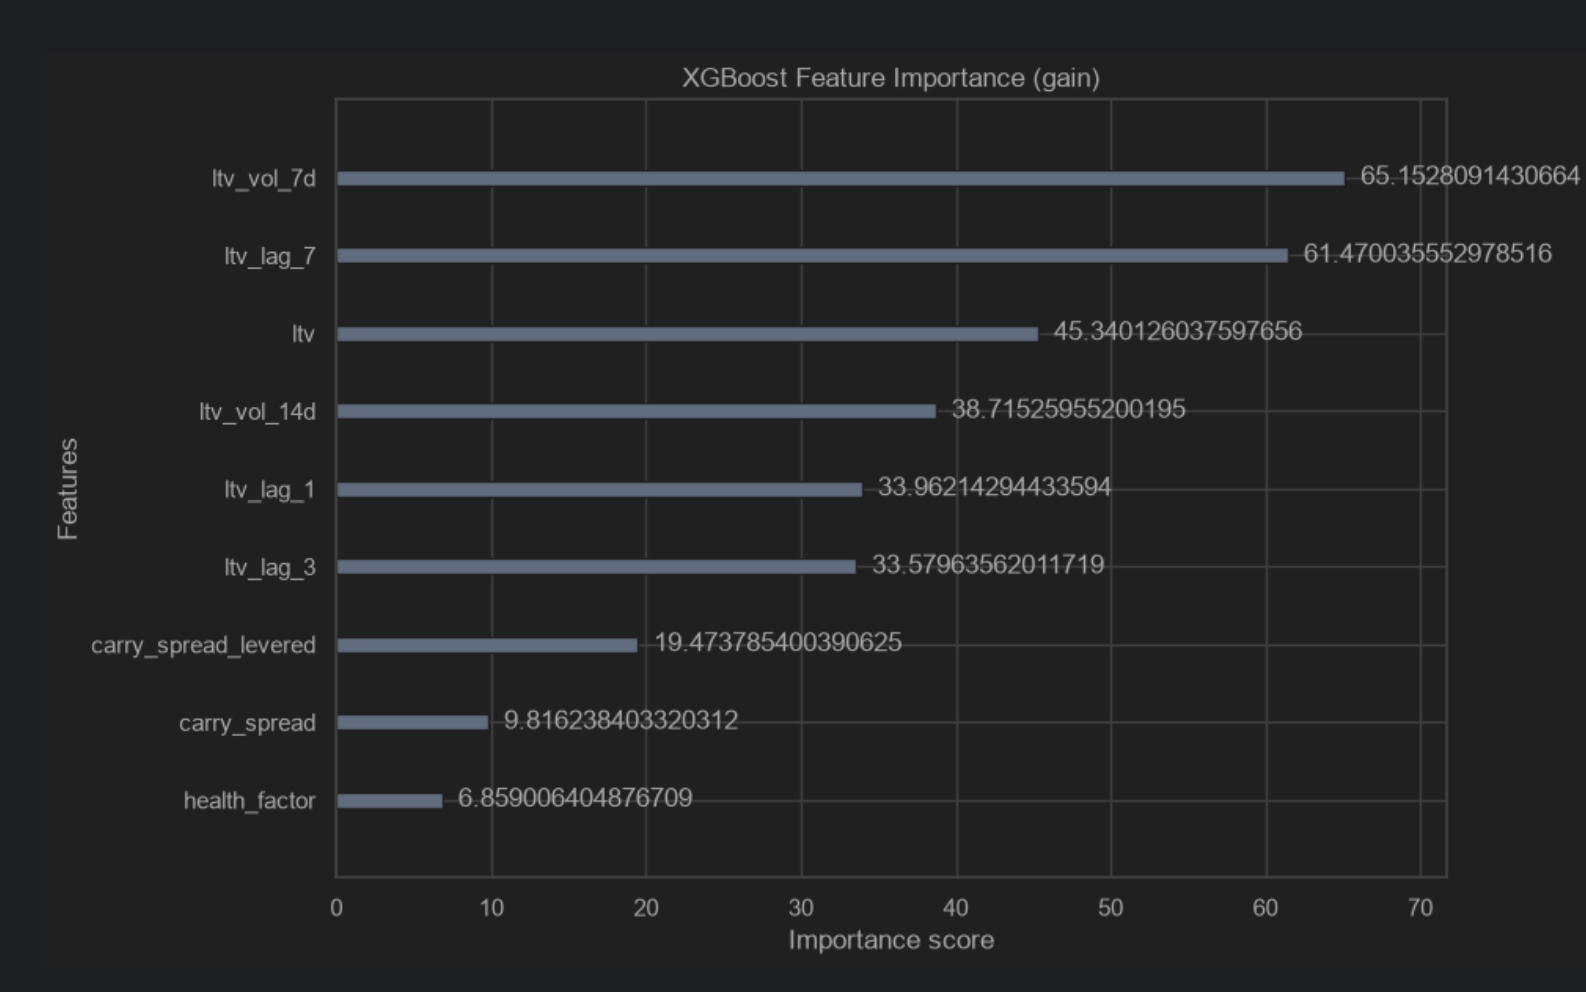
\includegraphics[width=0.9\textwidth]{figures/supervised/rebalance-xgb-feature-importance.png}
\caption{Gain-based feature importance for the XGBoost rebalancing model.
Bars show each feature's total gain (the improvement it contributes to
the split criterion) summed across all trees. LTV volatility
(\texttt{ltv\_vol\_7d}) and lagged LTV (\texttt{ltv\_lag\_7}) rank
highest; carry features and health factor rank lowest. Two features
(\texttt{distance\_to\_liq}, \texttt{loop\_depth}) were never used by any
tree and do not appear in the chart.}
\label{fig:rebal-gain}
\end{figure}

\begin{figure}[t]
\centering
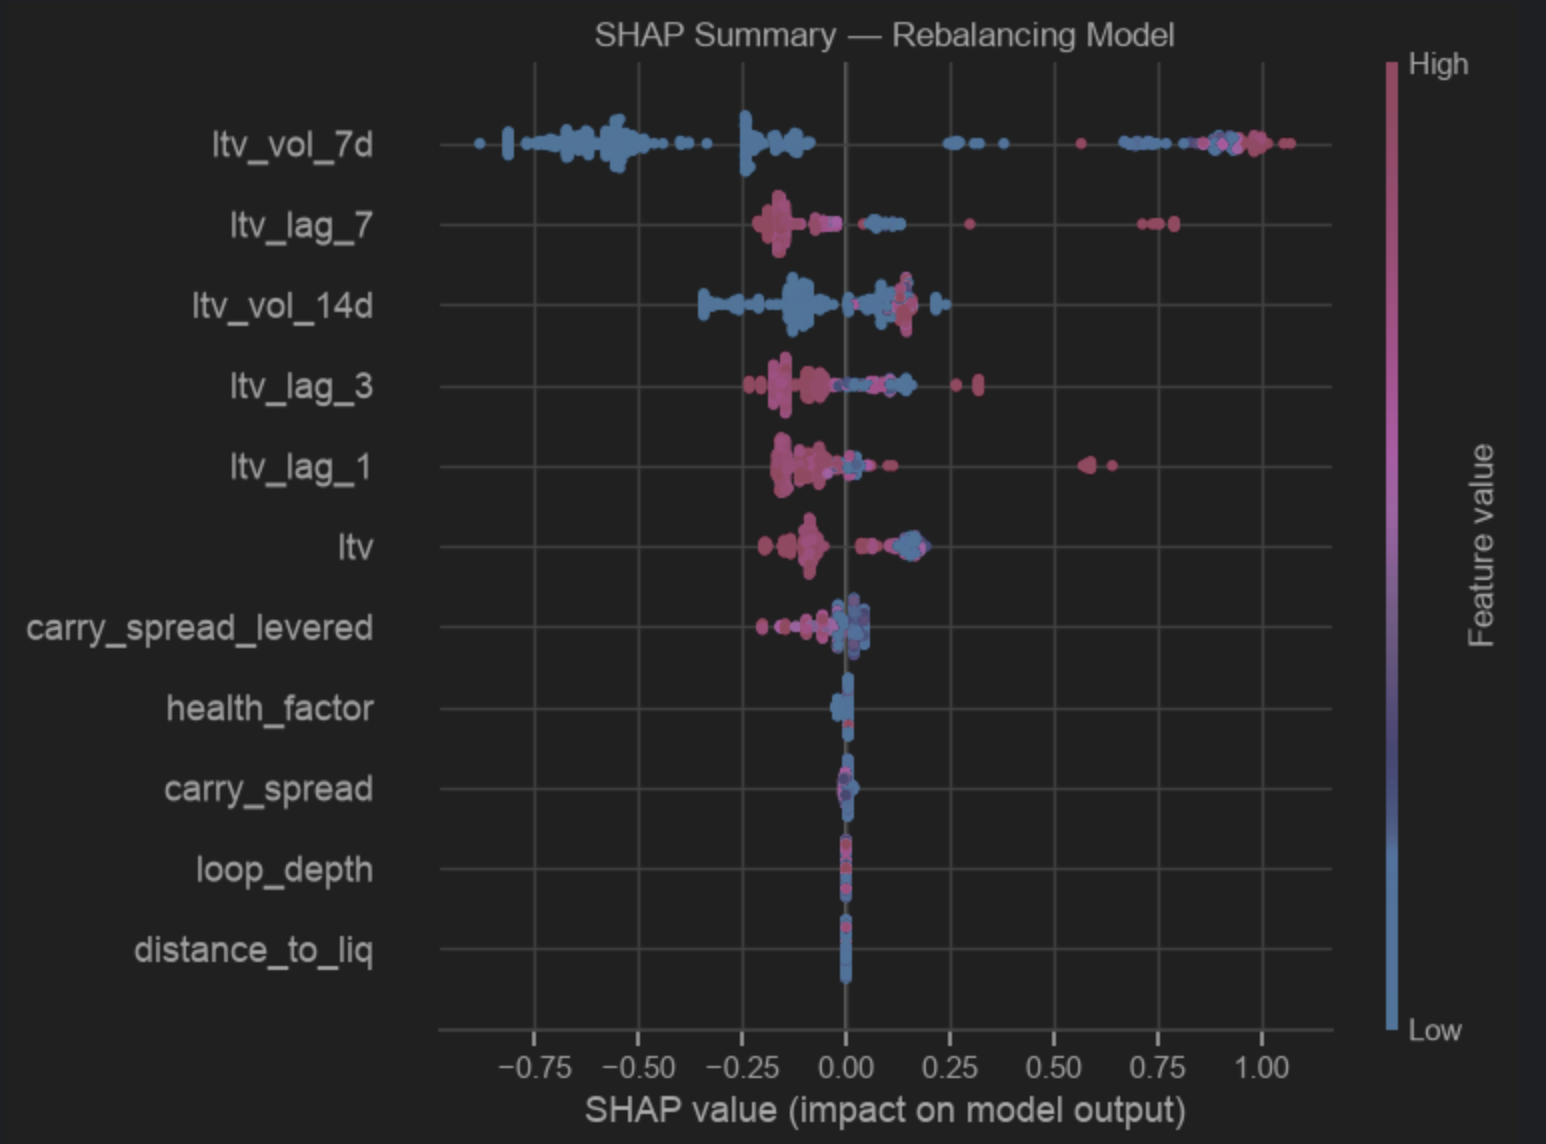
\includegraphics[width=0.9\textwidth]{figures/supervised/rebalance-shap.png}
\caption{SHAP summary for the XGBoost rebalancing model. Each point is a
whale-day; its horizontal position is the feature's signed contribution
to the predicted log-odds of rebalancing, and colour encodes the feature
value (red high, blue low). Features are ordered by mean absolute SHAP
value. High lagged LTV and high short-window LTV volatility push
predictions towards rebalancing, while the carry features and health
factor contribute little.}
\label{fig:rebal-shap}
\end{figure}

\subsubsection{Model B: Predicting Stressed States}
\label{sec:model-stressed}

Model~B predicts whether a whale is in a stressed risk state on a given
day using 9 features: LTV volatility (\texttt{ltv\_vol\_7d},
\texttt{ltv\_vol\_14d}), carry spread (raw and levered), yield and
interest rate variables (\texttt{ybt\_apy}, \texttt{borrow\_rate},
\texttt{supply\_rate}), and token prices (\texttt{collateral\_price},
\texttt{borrow\_price}). The feature set differs from Model~A because
several variables that are safe to use when predicting rebalancing
(such as \texttt{ltv}, \texttt{health\_factor}, and
\texttt{loop\_depth}) are too closely tied to the definition of
\texttt{stressed\_state} and would cause data leakage, as described in
Section~\ref{sec:ml-setup}.

After dropping rows with missing features, the modelling set is 2{,}088
rows; a stratified $70/30$ split gives 1{,}460 training and 628 test
observations. We evaluate both classifiers at two decision thresholds,
the default $0.5$ and a lowered $0.3$, and report all four
configurations in Table~\ref{tab:model-b}.

\begin{table}[t]
\centering
\caption{Model~B: stressed-state prediction across both classifiers and
both decision thresholds. ROC-AUC is threshold-independent and so repeats
within each model. The selected configuration (XGBoost at $t=0.3$) is
shown in bold.}
\label{tab:model-b}
\begin{tabular}{llcccc}
\hline
Model & $t$ & ROC-AUC & Recall & Precision & Accuracy \\
\hline
Logistic Regression & 0.5 & 0.971 & 0.95 & 0.75 & 0.89 \\
Logistic Regression & 0.3 & 0.971 & 0.98 & 0.67 & 0.84 \\
XGBoost             & 0.5 & 0.977 & 0.82 & 0.93 & 0.92 \\
\textbf{XGBoost}    & \textbf{0.3} & \textbf{0.977} & \textbf{0.90} & \textbf{0.81} & \textbf{0.90} \\
\hline
\end{tabular}
\end{table}

\paragraph{Choice of decision threshold.}
By default a classifier labels a day as stressed only when its predicted
probability exceeds $0.5$. We lower this threshold to $0.3$ so that the
model raises a flag whenever it is at least $30\%$ confident, catching
more stressed days at the cost of some false alarms. This trade-off is
deliberate: in a risk-monitoring setting a missed stressed day is far
more costly than a false alarm, since an unflagged stressed whale may
proceed to liquidation, whereas a false alarm merely prompts an
unnecessary check. Lowering the threshold therefore prioritises recall,
which is the quantity that matters most for this task.

\paragraph{Choice of model.}
The two classifiers behave differently at the lower threshold. Logistic
regression at $t=0.3$ achieves the highest recall ($0.98$) but at the
cost of precision: only $0.67$ of its stress predictions are correct, and
accuracy falls to $0.84$. XGBoost at $t=0.3$ reaches a recall of $0.90$
(catching 180 of 199 stressed days, missing only 19) while retaining a
precision of $0.81$ (with 42 false alarms out of 429 non-stressed days)
and an accuracy of $0.90$, alongside a stronger ROC-AUC ($0.977$ versus
$0.971$). XGBoost therefore identifies stressed states from their
underlying structure rather than by widening its positive predictions
indiscriminately, and we adopt it at $t=0.3$ as the final stressed-state
model.

With this configuration fixed, the gain-based feature importance
(Figure~\ref{fig:stress-gain}) and the SHAP summary
(Figure~\ref{fig:stress-shap}) show that stress is driven primarily by
yield and interest rate conditions rather than by leverage alone.
\texttt{ybt\_apy} ($89.3$) ranks first, followed closely by
\texttt{carry\_spread} ($84.5$), \texttt{supply\_rate} ($82.8$), and
\texttt{carry\_spread\_levered} ($71.8$). LTV volatility
(\texttt{ltv\_vol\_7d} at $69.6$, \texttt{ltv\_vol\_14d} at $41.3$) and
\texttt{borrow\_rate} ($40.2$) also contribute, but less than the yield
features. \texttt{collateral\_price} ($32.6$) and
\texttt{borrow\_price} ($28.2$) rank lowest, though neither is close to
zero. Importantly, no single feature dominates the way that
\texttt{ltv} or \texttt{loop\_depth} did in the leaking models, which
supports the conclusion that this result is genuine.

The SHAP summary confirms the direction of these effects.
\texttt{carry\_spread\_levered} has the widest spread (roughly $-1.5$ to
$1.5$): high values push strongly toward stress, while low values push
away from it. For \texttt{ybt\_apy} and \texttt{supply\_rate}, low values
(blue dots) push toward stress, consistent with the idea that falling
yields make a position more vulnerable. The volatility features show a
smaller rightward pull, meaning they add some signal but less than the
yield features.

\begin{figure}[t]
\centering
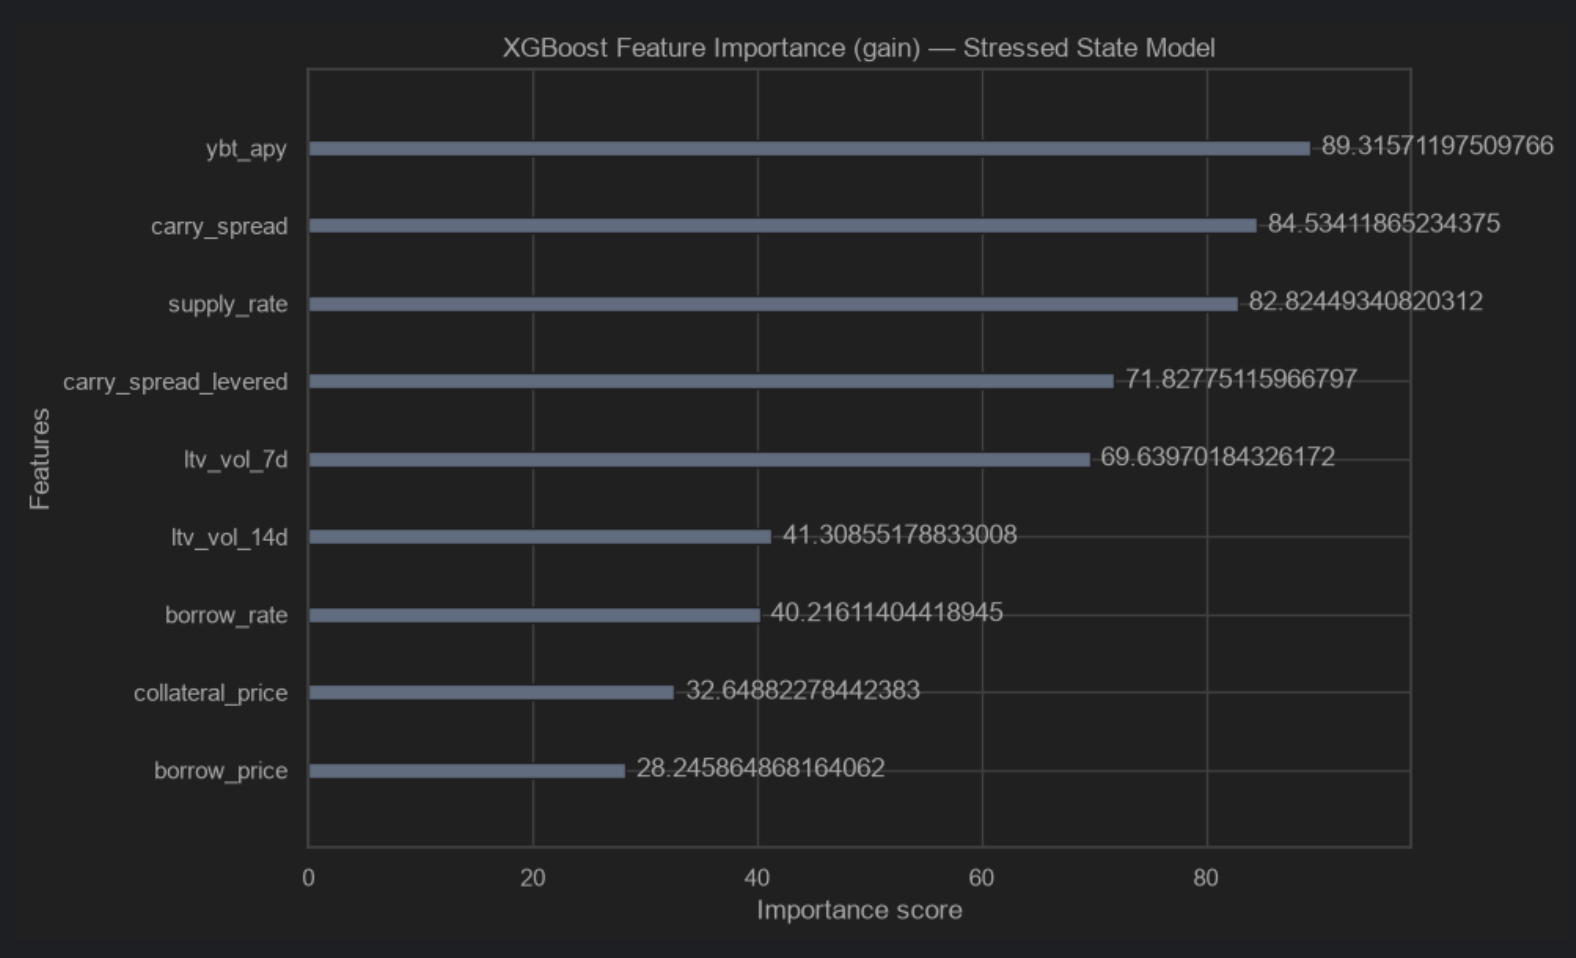
\includegraphics[width=0.9\textwidth]{figures/supervised/stress-feature-importance.png}
\caption{Gain-based feature importance for the XGBoost stressed-state
model. Bars show each feature's total gain summed across all trees. Yield
and rate features (\texttt{ybt\_apy}, \texttt{carry\_spread},
\texttt{supply\_rate}) rank highest; price features rank lowest. No
single feature dominates, and the label-defining features
(\texttt{health\_factor}, \texttt{distance\_to\_liq}) along with other
leaking variables are excluded.}
\label{fig:stress-gain}
\end{figure}

\begin{figure}[t]
\centering
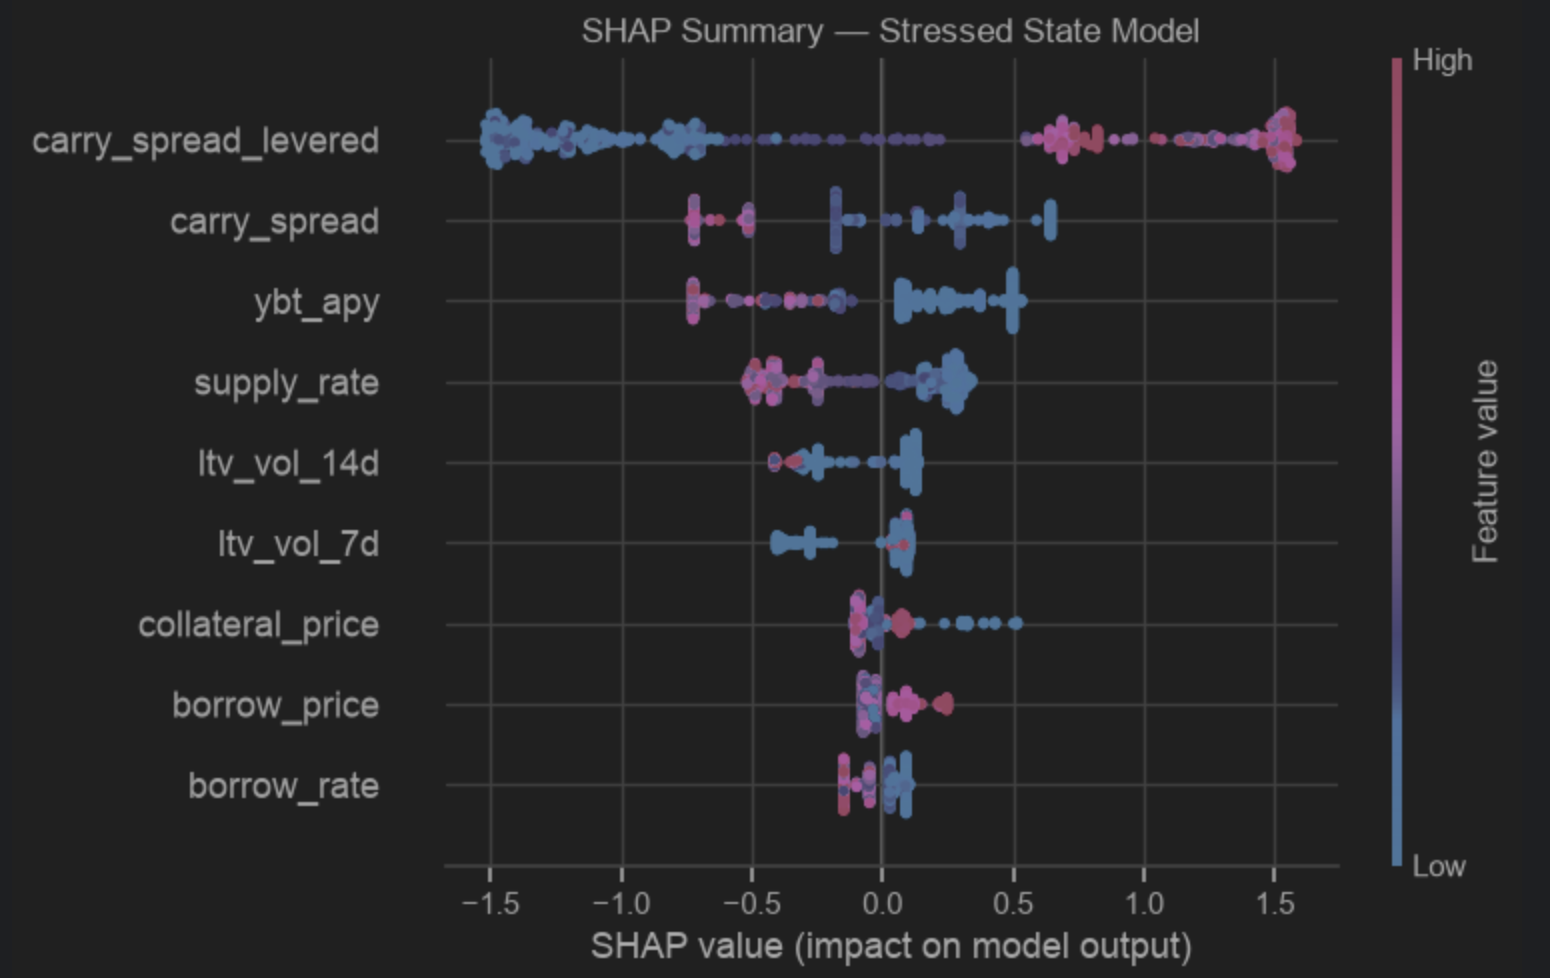
\includegraphics[width=0.9\textwidth]{figures/supervised/stress-shap.png}
\caption{SHAP summary for the XGBoost stressed-state model. Each point is
a whale-day; its horizontal position is the feature's signed contribution
to the predicted log-odds of being stressed, and colour encodes the
feature value (red high, blue low). Features are ordered by mean absolute
SHAP value. \texttt{carry\_spread\_levered} has the widest spread; low
yield (\texttt{ybt\_apy}) and low supply rate push predictions toward
stress.}
\label{fig:stress-shap}
\end{figure}

\subsubsection{Findings}
\label{sec:ml-findings}

Taken together, the two models give a clear answer to RQ3: on-chain state
variables can predict both rebalancing and stress, but through different
mechanisms.

\paragraph{Rebalancing is a delayed response.}
Whales do not rebalance the moment risk rises. The strongest predictors
of rebalancing are LTV volatility over the past week and lagged LTV
values rather than the current level, which indicates that operators
watch leverage accumulate and fluctuate over several days before acting.
Rebalancing therefore looks like a considered decision rather than a
panic reaction.

\paragraph{Stress tracks yield and rate conditions.}
The stressed-state model achieves strong detection (ROC-AUC of $0.977$,
recall of $0.90$ at threshold $0.3$) using only yield, rate, volatility,
and price features, without any direct leverage or structural variables.
The dominant predictors are \texttt{ybt\_apy}, \texttt{carry\_spread},
and \texttt{supply\_rate}. This suggests that a whale is more likely to
be in a stressed state when the yield it earns drops too close to its
borrowing cost, rather than simply when leverage is high. Stress in this
dataset looks less like ``leverage got too high'' and more like ``the
position stopped being worth the risk.''

\paragraph{Leverage volatility matters for both, but plays different
roles.}
In the rebalancing model, \texttt{ltv\_vol\_7d} is the single most
important feature. In the stressed-state model, it still matters but
ranks behind the yield and rate features. This suggests that volatility
is more of a trigger for action (rebalancing) than a marker of danger
(stress) in this dataset.

\paragraph{The broader picture.}
Whales appear to watch leverage build up over time before deciding to
rebalance, while their stressed state on any given day is shaped more
by yield and rate conditions than by leverage swings alone. On-chain
data captures both of these patterns clearly, which means that DeFi
leverage risk can likely be monitored, and to some extent anticipated,
in real time using only publicly available blockchain data. This is
directly relevant to on-chain risk monitoring and protocol parameter
calibration.
\section{Discussion}
\label{sec:discussion}

% TODO: Add findings discussion after analysis is complete.

\subsection{PT Looping: A Related Strategy Variant}

During whale identification, several addresses were found executing a structurally related but analytically distinct strategy using Pendle Principal Tokens (PT-sUSDe) as collateral rather than sUSDe directly. These are documented here for completeness but excluded from the core quantitative analysis.

\textbf{How Pendle works.} Pendle Finance splits a yield-bearing token into two components: a Principal Token (PT) redeemable for the underlying at a fixed maturity date, and a Yield Token (YT) that captures floating yield until maturity. Because the PT has been stripped of its yield, it trades at a discount implying a fixed annualised return for holders who hold to maturity.

\textbf{PT looping mechanism.} PT loopers use PT-sUSDe as Morpho collateral: obtain sUSDe, split via Pendle Router to receive PT-sUSDe and YT-sUSDe, supply PT-sUSDe as collateral on Morpho Blue, borrow stablecoin against it, convert borrowed stablecoin back to sUSDe, and repeat. The carry spread is the PT implied fixed rate minus the borrow rate, locked in at entry rather than floating daily.

\textbf{Why PT looping is excluded.}

\begin{table}[h!]
\centering
\caption{Comparison of YBT looping versus PT looping.}
\label{tab:pt-comparison}
\begin{tabular}{lp{4.5cm}p{4.5cm}}
\hline
\textbf{Dimension} & \textbf{YBT Looping (this study)} & \textbf{PT Looping (excluded)} \\
\hline
Collateral & Floating-rate YBT & Fixed-rate PT \\
Carry spread & Changes daily & Locked at entry \\
Price trajectory & Varies with yield & Predetermined accretion to par \\
Liquidation driver & YBT depeg or rate spike & PT price deviation from fair value \\
Panel structure & Continuous & Breaks at maturity \\
\hline
\end{tabular}
\end{table}

The maturity breaks are the primary engineering challenge. Each PT expiry requires special panel handling that does not apply to floating-rate positions. Combined with the need for Pendle AMM implied rate data (a separate API), this represents meaningful scope expansion.

Two PT loopers were identified during screening: an institutional-scale operator (\texttt{0x1b82b4f4...}) moving \$28--34M per atomic transaction with only 6 total transactions, and an iterative looper (\texttt{0xbfb77183...}) with 34 transactions concentrated in a two-day burst. Both are excluded from the core sample but demonstrate that recursive leverage extends beyond floating-rate YBTs into fixed-rate Pendle derivatives.

PT looping occupies a different position in the risk-return space: operators trade floating carry exposure for a predetermined fixed return. This places PT looping closer to fixed-income arbitrage than to the yield farming strategies analysed here, and represents a natural direction for future work.

\subsection{Limitations}

The most important limitation of the present analysis is the small number
of whales. With only seven wallets, several archetypes are dominated by a
single whale, most notably the extreme-leverage archetype, which is almost
entirely one wallet (W-2). Archetype and wallet identity are therefore
partially confounded, and the precise risk ordering between archetypes
should be regarded as provisional rather than settled. A larger and more
diverse set of wallets would be needed to establish whether the archetypes
generalise beyond individual operators.

This sample limitation also affects the stress comparison of
Section~\ref{sec:stress-by-archetype}. Because the supervised
\texttt{stressed\_state} label is defined relative to each whale's own
health-factor distribution, the stressed share of an archetype depends on
its wallet composition; this is why the per-whale label understates the
extreme-leverage archetype, which has no calm baseline of its own to stand
out against. We mitigate this by reporting an absolute health-factor
cut-off applied identically to every whale, but the cut-off itself is a
hand-picked buffer rather than one calibrated to observed liquidation
events. With more whales we would expect the two measures to converge, and
calibrating the absolute threshold to realised liquidations is left for
future work.

Further limitations shared with the supervised analysis include the
approximation of loop depth from observable position data and the
restriction to two lending protocols over a roughly seventeen-month window,
which together bound how far the archetype taxonomy can be generalised.

\section{Conclusions}
\label{sec:conclusions}

% TODO: To be completed at the end.


%\newpage
\bibliographystyle{splncs04}
\bibliography{main}

\appendix
\section{Glossary and Addresses}
\label{sec:glossary}

\subsection*{Whale Addresses}

\begin{tabular}{ll}
\hline
\textbf{ID} & \textbf{Address} \\
\hline
W-1 & \texttt{0x080ccea8654fd4ff80b81e46cff2278689d88fb0} \\
W-2 & \texttt{0x97bb0e08b664f65f05e0cff03b68bc1238b2e21e} \\
W-3 & \texttt{0xcb1effb6f6e531137ccc1508a8d4982e873aee58} \\
W-4 & \texttt{0x0d4f7b204626e8233c5b42b1269a78e236e9a06b} \\
W-5 & \texttt{0x24385a793f725328d7f6224430e48b4236326717} \\
W-6 & \texttt{0x029469ca80e6c94436af010a369f54935a711080} \\
W-7 & \texttt{0x24201ecd8b3f062215640b8c0740c4e892c091e3} \\
\hline
\end{tabular}

\subsection*{Glossary}

\begin{tabular}{p{3.5cm} p{9cm}}
\hline
\textbf{Term} & \textbf{Definition} \\
\hline
YBT & Yield-Bearing Token. A token that automatically earns yield (e.g., sUSDe, sUSDS, syrupUSDC). \\
Looping & Recursive leverage: deposit collateral, borrow, buy more collateral, repeat. \\
LTV & Loan-to-Value ratio. Borrowed amount divided by collateral value. \\
LLTV & Liquidation LTV. The threshold where a position gets liquidated. \\
Flashloan & Borrow and repay in the same transaction with no collateral required. \\
Morpho Blue & A lending protocol with isolated markets for each collateral-borrow pair. \\
Aave v3 & A pooled lending protocol with shared liquidity across assets. \\
Gnosis Safe & Multi-signature wallet requiring M-of-N signers to approve transactions. \\
ERC-4626 & Standard interface for yield-bearing vaults defining deposit, redeem, and share conversion. \\
The Graph & Decentralised indexing protocol for querying blockchain events via GraphQL. \\
Dune Analytics & SQL-based blockchain analytics platform. \\
Whale & Large holder, typically defined by total value received. \\
EOA & Externally Owned Account. A wallet controlled by a private key (vs smart contract). \\
Carry spread & Yield earned minus borrow cost. Positive means profitable loop. \\
Rebalancing & Any action that changes LTV (add/remove collateral, borrow/repay). \\
\hline
\end{tabular}

\section{Smart Contract Code}
\label{sec:code}

The following is the complete \texttt{LeverageBot.sol} contract deployed on Base mainnet.

\begin{verbatim}
// SPDX-License-Identifier: MIT
pragma solidity ^0.8.20;

import "./ILeverageBot.sol";

contract LeverageBot is IMorphoFlashLoanCallback {
    address public constant MORPHO = 0xBBBBBbbBBb9cC5e90e3b3Af64bdAF62C37EEFFCb;
    address public constant USDC = 0x833589fCD6eDb6E08f4c7C32D4f71b54bdA02913;
    address public constant YO_USD = 0x0000000f2eB9f69274678c76222B35eEc7588a65;

    address public constant MARKET_ORACLE = 0x77f59C5C09e7ABEF6991B456170930324FE36222;
    address public constant MARKET_IRM = 0x46415998764C29aB2a25CbeA6254146D50D22687;
    uint256 public constant MARKET_LLTV = 915000000000000000;
    bytes32 public constant MARKET_ID = 
        0x1a3e69d0109bb1be42b80e11034bb6ee98fc466721f26845dc83b2aa8d979137;

    uint256 public constant OWN_CAPITAL = 10_000_000;      // 10 USDC
    uint256 public constant FLASHLOAN_AMOUNT = 90_000_000; // 90 USDC

    uint8 private constant ACTION_LEVERAGE = 1;
    uint8 private constant ACTION_UNWIND = 2;

    address public owner;
    uint256 private _unwindUsdcReceived;

    modifier onlyOwner() {
        require(msg.sender == owner, "LeverageBot: not owner");
        _;
    }

    modifier onlyMorpho() {
        require(msg.sender == MORPHO, "LeverageBot: caller not Morpho");
        _;
    }

    constructor() {
        owner = msg.sender;
    }

    function execute() external onlyOwner {
        IERC20(USDC).transferFrom(msg.sender, address(this), OWN_CAPITAL);
        bytes memory data = abi.encode(ACTION_LEVERAGE, OWN_CAPITAL, FLASHLOAN_AMOUNT);
        IMorpho(MORPHO).flashLoan(USDC, FLASHLOAN_AMOUNT, data);
    }

    function onMorphoFlashLoan(
        uint256 flashloanAmount,
        bytes calldata data
    ) external override onlyMorpho {
        uint8 action = abi.decode(data, (uint8));
        if (action == ACTION_LEVERAGE) {
            _onLeverage(flashloanAmount, data);
        } else if (action == ACTION_UNWIND) {
            _onUnwind(flashloanAmount, data);
        }
        IERC20(USDC).approve(MORPHO, flashloanAmount);
    }

    function unwind() external onlyOwner {
        Position memory pos = IMorpho(MORPHO).position(MARKET_ID, address(this));
        require(pos.borrowShares > 0 || pos.collateral > 0, 
            "LeverageBot: no position");
        uint256 owedAssets = _debtSharesToAssets(pos.borrowShares);
        uint256 flashAmt = (owedAssets * 10100) / 10000 + 1;
        _runUnwindFlashloan(flashAmt, pos);
        uint256 netToOwner = IERC20(USDC).balanceOf(address(this));
        if (netToOwner > 0) {
            IERC20(USDC).transfer(owner, netToOwner);
        }
    }

    function transferOwnership(address newOwner) external onlyOwner {
        require(newOwner != address(0), "LeverageBot: zero owner");
        owner = newOwner;
    }

    function _onLeverage(uint256 flashloanAmount, bytes calldata data) private {
        (, uint256 ownCapital, ) = abi.decode(data, (uint8, uint256, uint256));
        uint256 totalUsdc = ownCapital + flashloanAmount;
        IERC20(USDC).approve(YO_USD, totalUsdc);
        uint256 yoUsdReceived = IERC4626(YO_USD).deposit(totalUsdc, address(this));
        MarketParams memory mp = _getMarketParams();
        IERC20(YO_USD).approve(MORPHO, yoUsdReceived);
        IMorpho(MORPHO).supplyCollateral(mp, yoUsdReceived, address(this), "");
        IMorpho(MORPHO).borrow(mp, flashloanAmount, 0, address(this), address(this));
    }

    function _onUnwind(uint256 flashloanAmount, bytes calldata data) private {
        (, uint256 borrowShares, uint256 collateral) = 
            abi.decode(data, (uint8, uint256, uint256));
        MarketParams memory mp = _getMarketParams();
        IERC20(USDC).approve(MORPHO, flashloanAmount);
        IMorpho(MORPHO).repay(mp, 0, borrowShares, address(this), "");
        IMorpho(MORPHO).withdrawCollateral(mp, collateral, address(this), address(this));
        uint256 yoUsdHeld = IERC20(YO_USD).balanceOf(address(this));
        if (yoUsdHeld > 0) {
            _unwindUsdcReceived = IERC4626(YO_USD).redeem(
                yoUsdHeld, address(this), address(this));
        }
    }

    function _getMarketParams() private pure returns (MarketParams memory) {
        return MarketParams({
            loanToken: USDC,
            collateralToken: YO_USD,
            oracle: MARKET_ORACLE,
            irm: MARKET_IRM,
            lltv: MARKET_LLTV
        });
    }
}
\end{verbatim}

The full source code including interfaces and tests is available in the project repository at \texttt{bot/contracts/}.

\section{SQL Queries}
\label{sec:queries}

The following Dune Analytics queries are used for data collection. Full SQL is available in the project repository.

\subsection*{YBT Price and Event Queries}

\begin{table}[h]
\centering
\begin{tabular}{ll}
\hline
\textbf{Data} & \textbf{Dune Query ID} \\
\hline
Daily prices & 7359293 \\
Aave v3 events (sUSDe) & 7359302 \\
Morpho Blue events (all tokens) & 7359324 \\
SparkLend events (sUSDS) & 7368610 \\
\hline
\end{tabular}
\end{table}

\subsection*{Whale Identification Queries}

\begin{table}[h]
\centering
\begin{tabular}{lll}
\hline
\textbf{Token} & \textbf{Protocol} & \textbf{Dune Query ID} \\
\hline
sUSDe & Aave v3 & 7349560 \\
sUSDe & Morpho Blue & 7344848 \\
sUSDS & Morpho Blue & 7367663 \\
sUSDS & SparkLend & 7368059 \\
syrupUSDC & Morpho Blue & 7367806 \\
\hline
\end{tabular}
\end{table}

\subsection*{Sample SQL: Aave v3 Events}

\begin{verbatim}
SELECT 
    'supply' AS event_type,
    evt_block_time AS block_time,
    evt_block_number AS block_number,
    evt_tx_hash AS tx_hash,
    "user",
    onBehalfOf AS on_behalf_of,
    'sUSDe' AS token,
    CAST(amount AS DOUBLE) / 1e18 AS amount
FROM aave_v3_ethereum.Pool_evt_Supply
WHERE reserve = 0x9D39A5DE30e57443BfF2A8307A4256c8797A3497

UNION ALL

SELECT 
    'withdraw' AS event_type,
    evt_block_time, evt_block_number, evt_tx_hash,
    "user", "to" AS on_behalf_of, 'sUSDe',
    CAST(amount AS DOUBLE) / 1e18
FROM aave_v3_ethereum.Pool_evt_Withdraw
WHERE reserve = 0x9D39A5DE30e57443BfF2A8307A4256c8797A3497

-- borrow, repay, liquidation events follow same pattern
ORDER BY block_time DESC
\end{verbatim}

\subsection*{Sample SQL: SparkLend Events}

\begin{verbatim}
SELECT 
    'supply' AS event_type,
    evt_block_time AS block_time,
    evt_block_number AS block_number,
    evt_tx_hash AS tx_hash,
    "user",
    onBehalfOf AS on_behalf_of,
    'sUSDS' AS token,
    CAST(amount AS DOUBLE) / 1e18 AS amount
FROM spark_protocol_multichain.pool_evt_supply
WHERE reserve = 0xa3931d71877C0E7a3148CB7Eb4463524FEc27fbD
  AND chain = 'ethereum'

-- withdraw, borrow, repay, liquidation follow same pattern
ORDER BY block_time DESC
\end{verbatim}

\subsection*{Sample SQL: Morpho Blue Events}

\begin{verbatim}
SELECT 
    'supply' AS event_type,
    evt_block_time AS block_time,
    evt_block_number AS block_number,
    evt_tx_hash AS tx_hash,
    onBehalf AS on_behalf_of,
    CASE JSON_EXTRACT_SCALAR(marketParams, '$.collateralToken')
        WHEN '0x9D39A5DE...7A3497' THEN 'sUSDe'
        WHEN '0xa3931d71...27fbD' THEN 'sUSDS'
        WHEN '0x80ac24aA...5Cc0b' THEN 'syrupUSDC'
    END AS token,
    CAST(assets AS DOUBLE) / 1e18 AS amount
FROM morpho_blue_ethereum.MorphoBlue_evt_SupplyCollateral
WHERE JSON_EXTRACT_SCALAR(marketParams, '$.collateralToken') IN (
    '0x9D39A5DE30e57443BfF2A8307A4256c8797A3497',
    '0xa3931d71877C0E7a3148CB7Eb4463524FEc27fbD',
    '0x80ac24aA929eaF5013f6436cdA2a7ba190f5Cc0b'
)

-- withdraw, borrow, repay, liquidation follow same pattern
ORDER BY block_time DESC
\end{verbatim}

All queries are available at \texttt{https://dune.com/queries/<ID>}. The complete SQL including borrow, repay, and liquidation events is documented in \texttt{data/ybt/README.md} and \texttt{data/whales/README.md}.


\end{document}
